\documentclass{ltjsarticle}
\title{{\bf Rの実習課題2} \\ パーセプトロン型学習回路とCNN}
\author{201611353 荻野夏樹}
\usepackage{graphicx}
\usepackage[unicode,bookmarksnumbered]{hyperref} %PDFで自動的に目次
%\usepackage{subfiles}
\usepackage{lastpage}
\usepackage{fancyhdr}
\usepackage{amsmath}
\usepackage{amssymb}
\usepackage{ascmac}
\usepackage{url}       % \urlでエスケープなしでurlを表示
\usepackage{listings}  % ソースコード
\usepackage{color}
\usepackage{here}      % figureで[H]を使えるようにする
\usepackage{mathtools} % 参照している式番号のみを表示
\usepackage{bm} % \bm{}でbold,italicでベクトルを表す
\usepackage{titlesec} % sectionの文字サイズを変更
\titleformat*{\section}{\large\bfseries}
%\titleformat*{\subsection}{\large\bfseries}
%\titleformat*{\subsubsection}{\large\bfseries}
\lstset{
	numbers=left,
	numbersep=1em,
%	numberstyle=\tiny\color{red}\noaccsupp,
	frame=single,
%	framesep=\fboxsep,
%	framerule=\fboxrule,
%	rulecolor=\color{red},
%	xleftmargin=\dimexpr\fboxsep+\fboxrule\relax,
%	xrightmargin=\dimexpr\fboxsep+\fboxrule\relax,
	breaklines=true,
	columns=flexible,
	basicstyle=\ttfamily\footnotesize,
	tabsize=4
}
\graphicspath{{../images/}} %実は相対パスで指定してる
%\nonumber
\mathtoolsset{showonlyrefs=true} % 参照している式番号のみを表示
%\renewcommand{\thesection}{(\arabic{section})}
%\renewcommand{\thesubsection}{(\arabic{section}--\arabic{subsection})}
\begin{document}
\maketitle
\section{誤差逆伝播学習アルゴリズム}
\subsection{レポート課題}

排他的論理和を誤差逆伝搬法で学習し、以下の問いに答えなさい。

\subsubsection{隠れ素子を一つずつ増やし、10 回の学習で 10 回とも正しく識別できるようになった隠れ素子の数を求めなさい。}
第1節に用いたソースコードを以下に示す。
実装の方針としては$40 \times 10$の二次元配列に学習済みモデルを代入するようにした。
\lstinputlisting[title=\url{xor.R}]{./xor.R}
\begin{lstlisting}
q1 <- function(){
	#<<-はグローバル変数に代入
	first_match <<- which(trave == 0)[1] #複数マッチするので一番初めを取り出す
	print(first_match)
}
\end{lstlisting}
{\bf q1()}を実行して{\bf first\_match}に初めて10回とも正しく識別できるようになった隠れ素子の数を格納し、表示したところ\\
34\\
であった。

\subsubsection{隠れ素子の数によって誤識別率の平均がどのように変化するかをグラフで示しなさい。}
\begin{lstlisting}
q2 <- function(){
	plot(hidden, trave, type="b")
	#	 , lty=1, lwd=2)
}
\end{lstlisting}
{\bf q2()}を実行して得られたグラフを以下に示す。
\begin{figure}[H]
	\centering
	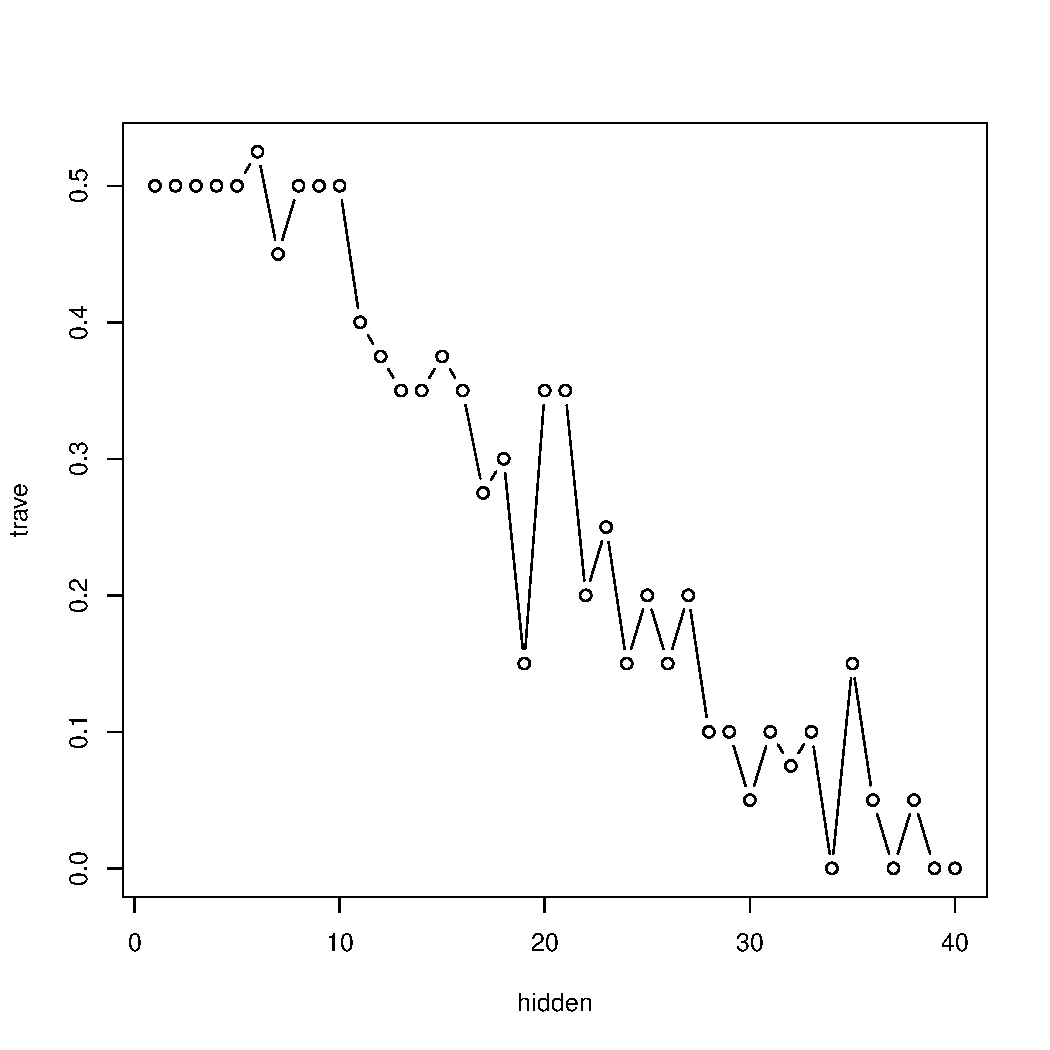
\includegraphics[width=0.5\hsize]{./fig1_2.pdf}
	\caption{隠れ素子の数と識別率の平均}
	\label{fig1_2}
\end{figure}
おおむね負の相関があるが分かった。
\subsubsection{隠れ素子が 1 個の場合に得られた学習結果について、結合係数の大きさの分布を示しなさい。}
学習した10個のモデルの内の1つ目のヒストグラムを以下に示す
\begin{figure}[H]
	\centering
	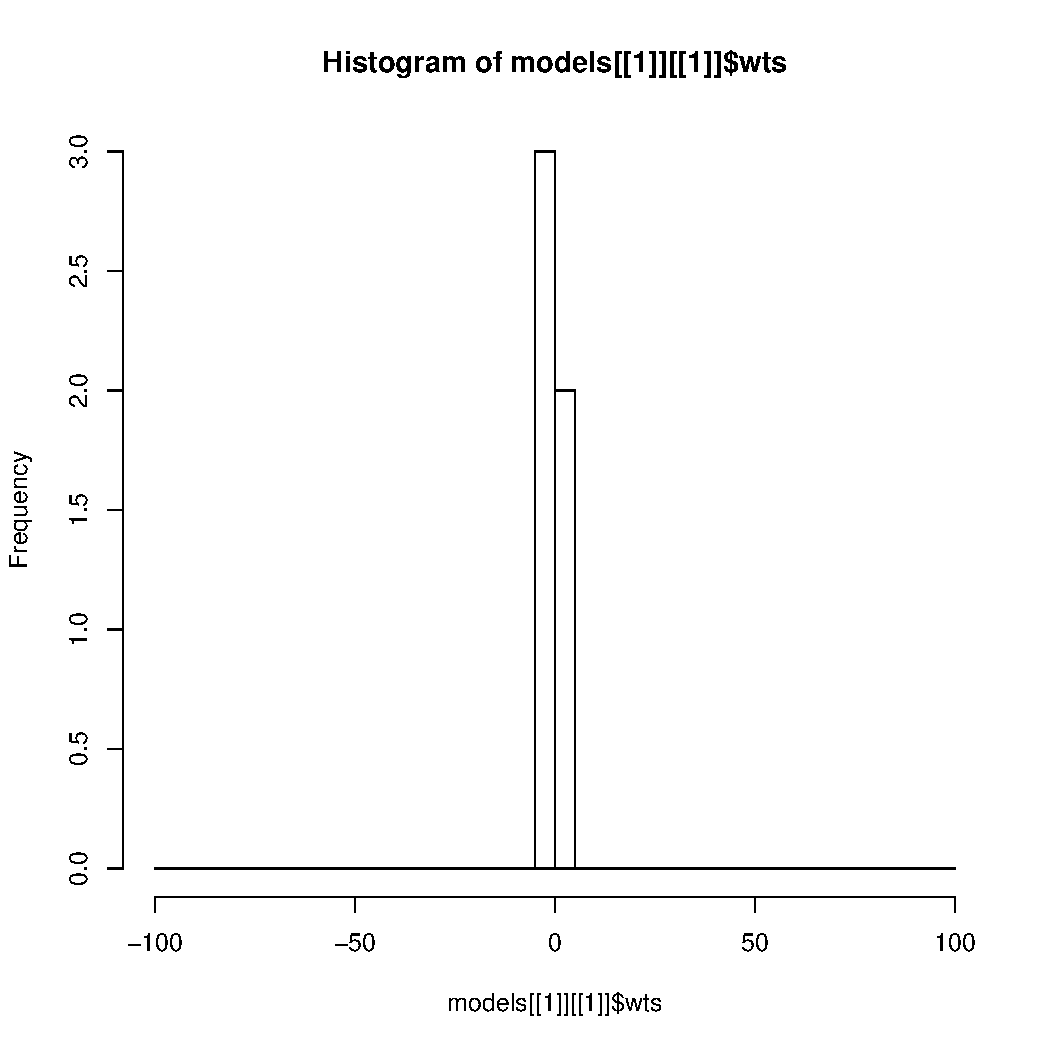
\includegraphics[width=0.5\hsize]{./fig1_3.pdf}
	\caption{隠れ素子が1個の場合の結合係数の大きさの分布}
	\label{fig1_3}
\end{figure}

\subsubsection{10 回とも正しく識別できた場合の学習結果について、結合係数の大きさの分布を示し、隠れ素子が1個の場合と 比較検討しなさい。}
10回学習したが1回目のモデルを用いた
\begin{figure}[H]
	\centering
	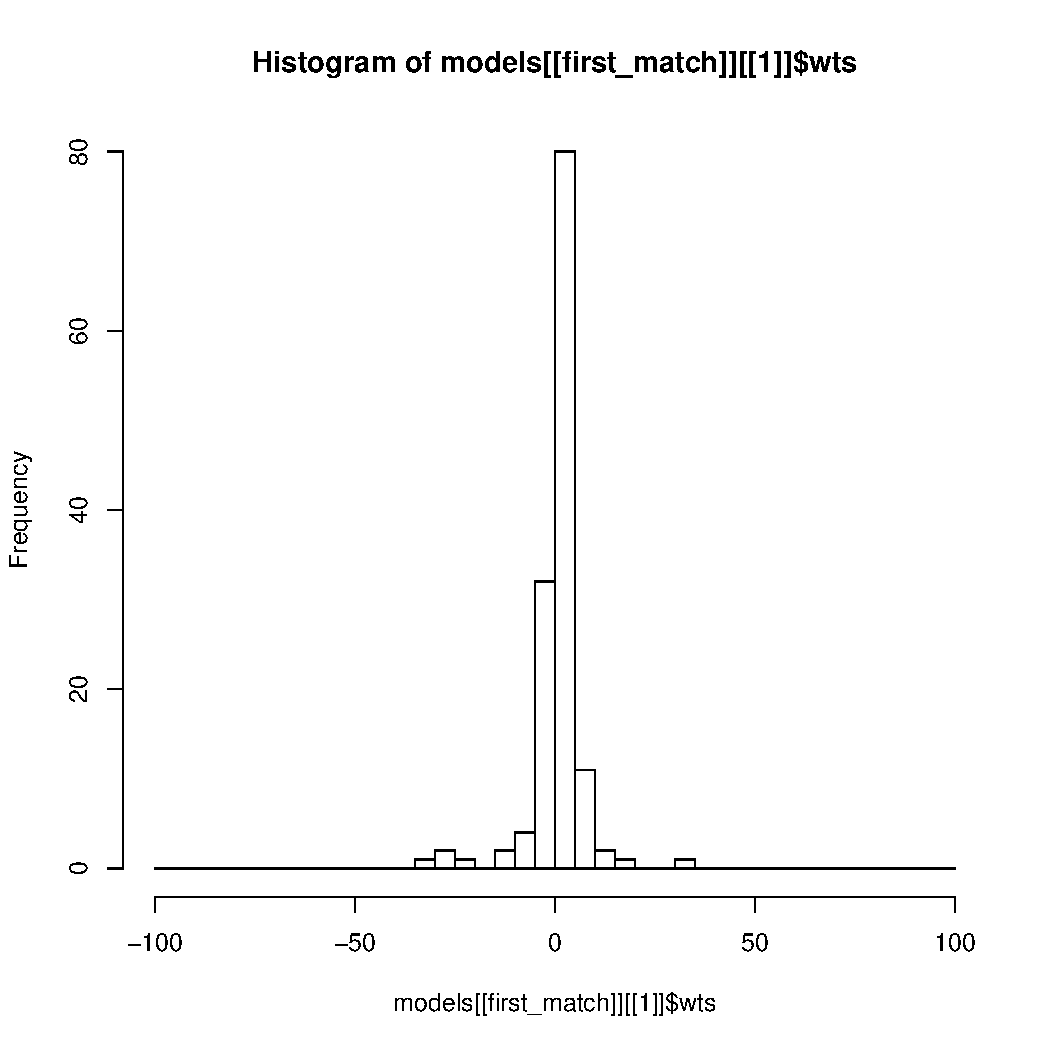
\includegraphics[width=0.5\hsize]{./fig1_4.pdf}
	\caption{隠れ素子がfirst\_match個の場合の結合係数の大きさの分布}
	\label{fig1_4}
\end{figure}


\subsection{レポート課題}

アヤメデータを用いて誤差逆伝搬法による学習を行い、下記の項目に答えなさい。

\subsubsection{decay=0 に設定し、隠れ素子の数を 1 にして学習データを用いて 10 回学習し、学習データに対する誤識別率の平均と、テストデータに対する誤識別率の平均を求めなさい。隠れ素子の数を 10 まで 1 つずつ増やして同じことを行い、隠れ素子の数に対する再代入誤りと汎化誤差の変化をグラフ化しなさい。}
第2節に用いたソースコードを以下に示す。
\lstinputlisting[title=\url{iris.R}]{iris.R}
\begin{figure}[H]
	\centering
	\includegraphics[width=0.5\hsize]{./images/1_2_1_1.png}
	\caption{隠れ素子の数に対する再代入誤りの変化}
\end{figure}
\begin{figure}[H]
	\centering
	\includegraphics[width=0.5\hsize]{./images/1_2_1_2.png}
	\caption{隠れ素子の数に対する汎化誤差の変化}
\end{figure}

\subsubsection{再代入誤りが一番小さな場合の結合係数の分布と、汎化誤差が一番小さな場合の結合係数の分布を比較検討しなさい。}
\begin{figure}[H]
	\centering
	\includegraphics[width=0.5\hsize]{./images/1_2_2_1.png}
	\caption{再代入誤りが一番小さな場合の結合係数の分布}
\end{figure}
\begin{figure}[H]
	\centering
	\includegraphics[width=0.5\hsize]{./images/1_2_2_2.png}
	\caption{汎化誤差が一番小さな場合の結合係数の分布を}
\end{figure}
ほぼ一致した。

\subsubsection{decay=0.01 にして同様の実験を行い、隠れ素子数に対する再代入誤りと汎化誤差の変化をグラフ化しなさい。}
\begin{figure}[H]
	\centering
	\includegraphics[width=0.5\hsize]{./images/1_2_3_1.png}
	\caption{隠れ素子数に対する再代入誤りの変化}
\end{figure}
\begin{figure}[H]
	\centering
	\includegraphics[width=0.5\hsize]{./images/1_2_3_2.png}
	\caption{隠れ素子数に対する汎化誤差の変化}
\end{figure}

\subsubsection{再代入誤りが一番小さな場合の結合係数の分布と、汎化誤差が一番小さな場合の結合係数の分布を、decay=0 の場合と 比較検討しなさい。}
\begin{figure}[H]
	\centering
	\includegraphics[width=0.5\hsize]{./images/1_2_4_1.png}
	\caption{再代入誤りが一番小さな場合の結合係数の分布}
\end{figure}
\begin{figure}[H]
	\centering
	\includegraphics[width=0.5\hsize]{./images/1_2_4_2.png}
	\caption{汎化誤差が一番小さな場合の結合係数の分布}
\end{figure}
ほぼ一致した。

\section{手書き数字認識}
%\subsection{レポート課題}
%
%例題に従って全結合型 3 層パーセプトロンによる手書き数字認識システムを実装し、下記の問いに答えなさい。
%
%\subsubsection{3 つの異なった乱数の種を用いて、学習データとテストデータに対する認識率を求めなさい。}
%
%\subsubsection{最初の二つの隠れ層の非線形出力関数をシグモイド関数 (sigmoid) にした場合、認識率はどのようになるか。ReLU の場合と同じ条件で実験し、比較しなさい。}
%
\section{CNNによる手書き文字認識システムの構成}
\subsection{レポート課題}

以下の問いでは、素子数の計算にバイアス素子は含めなくてよい。

\subsubsection{第 1 隠れ層の conv1 の出力素子数は M1 × M1 × N1 である。また、pool1 の出力素子数は M2 × M2 × N2 である。M1 , N1 と M2 , N2 はいくつか。}
$M1=24,N1=20,M2=12,N2=20$

\subsubsection{第 2 隠れ層の conv2 の出力素子数は M3 × M3 × N3 である。また、pool2 の出力素子数は M4 × M4 × N4 である。M3 , N3 と M4 , N4 はいくつか。}
$M3=8,N3=50,M4=4,N4=50$

\subsubsection{第 1 全結合層への入力を作っている mx.symbol.Flatten() 関数の役割は何か。}
4次元の配列をx, y, filterをまとめるて2次元配列にしている。
\subsection{学習データとテストデータに対する正答率はいくつになったか。}

\subsection{dropout 正則化を外した場合、学習データとテストデータに対する正答率はいくつになったか。}

\subsection{dropout 正則化を外した状態で、出力関数を tanh から ReLU に変えた場合、学習データとテストデータに対する正答率はいくつになったか。}

\subsection{dropout 正則化と ReLU を用いた場合、学習データとテストデータに対する正答率はいくつになったか。}

\subsection{以上の比較実験から、dropout 正則化は有効といえるか。また、出力関数はどちらがよいといえるか。}

\subsection{以上の中で、テストデータに対する正答率が最も良い組み合わせのネットワークに Kaggle の学習データで学習させなさい。Kaggle のテストデータに対する識別結果を下記の手順で作成し、Kaggle に submit しなさい。正答率と順位はいくつになったか。}
\end{document}
